\chapter{Method Validation} \label{chap:validation} \minitoc

\section{Datasets}

In order to test our proposed system, we generated multiple synthetic datasets before moving on to real data. As an initial first step we started by validating our system using a single-feature dataset before moving to multi-feature scenarios in order to facilitate system validation considering the complexities of multi-feature datasets and the problem of multiple test correction.


\begin{table}[!htb]
    \begin{center}
        \begin{tabular}{|c|c|c|}
        \hline
        \textbf{Dataset} & \textbf{Features} & \textbf{Events} \\ \hline
        R1               & 1                 & 5.000.000       \\ \hline
        T1               & 1                 & 5.000.000       \\ \hline
        
        \end{tabular}
    \end{center}
    \caption{Summary statistics for each dataset}
    \label{tbl:summary-statistics}
\end{table}

\subsection{Synthetic datasets}
Dataset R1 had a single feature that followed a normal distribution with mean $\mu=10$ and $\sigma=2$ for the entirety of the dataset. Figure \ref{fig:timeseries-r1} shows the time-series of the single feature in dataset R1.

\begin{figure}[!htb]
    \begin{center}
      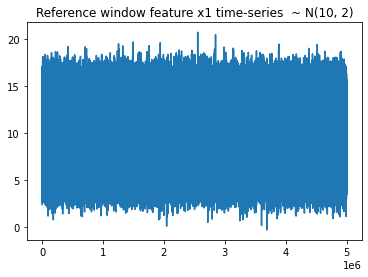
\includegraphics[scale=0.6]{figures/01-reference.png}
      \caption[]{Time-series for dataset R1}
      \label{fig:timeseries-r1}
    \end{center}
\end{figure}


Dataset T1 also had 5 million events with a single feature. For the first half, \textit{i.e.}, for the first 2.5 million events, the feature followed a normal distribution with mean $\mu=10$ and $\sigma=2$. For the other half, we changed the generating distribution to be a continuous uniform one with $a=100$ and $b=200$. Figure \ref{fig:timeseries-t1} shows the time-series of the single feature in dataset T1 where we see the abrupt change in feature values.

\begin{figure}[!htb]
    \begin{center}
      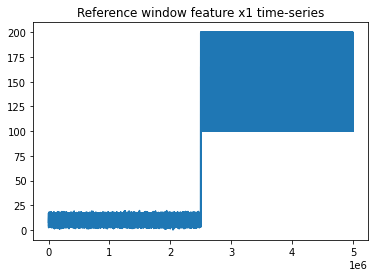
\includegraphics[scale=0.6]{figures/01-target.png}
      \caption[]{Time-series for dataset T1}
      \label{fig:timeseries-t1}
    \end{center}
\end{figure}



\subsection{Financial fraud datasets}

\section{Experiments}
\textcolor{red}{one subsection per experiment with i) purpose, ii) execution, iii) results obtained and what thye mean}

\subsection{Single-feature analysis with varying sample sizes}
In this first experiment, we used dataset R1 as the reference period and dataset T1 as the target or streaming period. We used 100 bins for the equal-height reference histogram and then added the two special bins mentioned in Section \ref{sec:sampling-batch}. We changed the half-life of each EMA-like sample histogram (recall Section \ref{sec:ema-hist}), effectively changing its size. We tested samples with \textit{(a)} 2.500, \textit{(b)} 250.000 and \textit{(c)} 1.000.000 events.

\textcolor{red}{We use tukey threshold, how do we introduce this, ahhhhhhhhhhhh}


\section{Conclusions}
